% !TeX spellcheck = hu_HU
\topic{Struktúra alapú modellezés}

\graphicspath{ {./struktura-alapu-modellezes/figures/} }

\newcommand{\yedscale}{0.7}

% vezérpélda lehetőségek
% - táblázatszerű adatok pl. felhasználókról (preferenciák, van-e jogsija, stb.), kocsikról (férőhely, légkondi stb.)
% - kiszolgáló rendszer top-down, bottom-up tervezése (mobil kliens, tömegközl. integráció, adatbázis stb.)
% - gráfként reprezentált fuvarok, kocsik, szakaszok, utasok, sofőrök stb.

%\begin{megjegyzes}
%	kifejteni azt, hogy lehet logikai és fizikai felépítés alapján is modellezni.
%
%	- Fizikai/architektúrális egységek --> moduláris struktúra hoz létre, újrahasznosítható részekkel.
%
%	- Funkcionális egységek --> dedikált struktúrát hoz létre, pl. távirányító -- redundanciamentes, azért, hogy a költség alacsony legyen. Nem újrahasznosíthatók a részei.
%
%	Pl. dedikált eszközt készítünk, amikor van egy rendszermenedzsment problémám és írok rá egy szkriptet. A másik megoldás lenne, hogy behozunk egy rendszermenedzsment eszközt és annak az újrahasznosítható komponenseit alkalmazzuk.
%
%	Jó lenne építészeti példát behozni.
%\end{megjegyzes}

Hogyan épül fel egy rendszer? Milyen részekre bontható és ezek között milyen kapcsolat van? Ahhoz, hogy a rendszerünkkel kapcsolatos problémákat megválaszoljuk, fontos, hogy ezekre a kérdésekre tudjuk a választ. Ebben a fejezetben az egyes rendszerek \fogalomragozva{struktura}{struktúrájának} jellemzésével foglalkozunk. Bemutatjuk a strukturális modellezés motivációját, a leggyakrabban alkalmazott formalizmusokat és azok matematikai alapjait.

%Modellezés során egy rendszert jellemezhetünk annak statikus, ill. dinamikus jellemzői alapján. A statikus jellemzés esetén a rendszer felépítését, \fogalomragozva{struktura}{struktúráját} írjuk le, míg dinamikus jellemzés esetén a rendszer \fogalomragozva{viselkedes}{viselkedésével} foglalkozunk.

%\clearpage

%%%%%%%%%%%%%%%%%%%%%%%%%%%%%%%%%%%%%%%%%%%%%%%%%%%%%%%%%%%%%%%%%%%%%%%%%%%%%%%%

\section{A strukturális modellezés alkalmazásai}
\label{sec:motivacio}

Mind a természetben, mind az ember alkotta rendszerekben fellelhetők bizonyos szabályszerűségek: egyesek a rendszer elemei közötti kapcsolatokat, míg mások magukat az elemeket jellemzik. Bár sok mindenben eltér egy közlekedési hálózat, egy számítógép-hálózat, egy épület vagy egy város felépítése, a strukturális modellezés eszköztárával olyan ,,nyelvet'' kapunk, amivel ezeket hasonlóan modellezhetjük.

\subsection{Hálózatok}
\label{sec:halozatok}

Egy rendszert gyakran úgy jellemezhetünk a legjobban, ha bizonyos elemeit megkülönböztetjük és leírjuk az ezek közötti \fogalomragozva{kapcsolat}{kapcsolatokat}.

\begin{pelda}
	Egy nagyváros közlekedése az autóutak és sínhálózatok, a százezernyi járműnek és a rajta utazó embereknek szövevényes rendszere. A közlekedők folyamatosan mozgása mellett az infrastruktúra is rendszeresen változik a különböző fejlesztések, átalakítások és karbantartások miatt.

	Egy ilyen rendszer precíz modellezése lehetetlen vállalkozás lenne, ezért helyette tipikusan olyan absztrakciókkal dolgozunk, amik az adott probléma megoldásához szükséges információkat tartalmazzák. Például az útvonalkereső alkalmazások ismerik a helyi tömegközlekedés járatait és segítséget nyújtanak abban, hogy az indulási pontunktól a célállomásig közlekedő járműveket és a közöttük lehetséges átszállásokat listázzák.

	Vizsgáljuk meg például Budapest metróhálózatát! Az egyszerűség kedvéért a példában a hálózatnak csak a Nagykörúton belüli részével foglalkozunk.
\end{pelda}

A metróhálózat egyszerűsített térképe \aref{fig:metrohalozat-nagykorut-terkep} ábrán látható. A térképből is látható, hogy a hálózat könnyen ábrázolható egy \fogalomragozva{graf}{gráffal}, ahol a gráf minden \fogalomragozva{csomopont}{csomópontja} egy-egy metróállomást jelöl. A csomópontok címkéje a metrómegálló neve. Két csomópont között akkor fut \fogalom{el}, ha a két megálló közvetlenül össze van kötve metróval (azaz nincs közöttük másik megálló). A metróhálózatot modellező %\fogalomragozva{iranyitatlan-graf}{irányítatlan}, \fogalomragozva{cimkezett-graf}{címkézett}, \fogalom{egyszeru-graf}
gráf \aref{fig:metrohalozat-nagykorut-egyszeru} ábrán látható.

\begin{figure}[H]
	\begin{subfigure}[b]{0.5\textwidth}
		\centering
		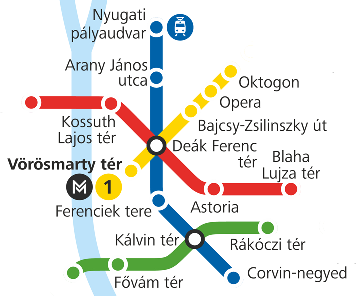
\includegraphics[width=0.9\textwidth]{metrohalozat-nagykorut-terkep}
		\caption{A metróhálózat térképe~\cite{BKK:metro}}
		\label{fig:metrohalozat-nagykorut-terkep}
	\end{subfigure}
	~
	\begin{subfigure}[b]{0.5\textwidth}
		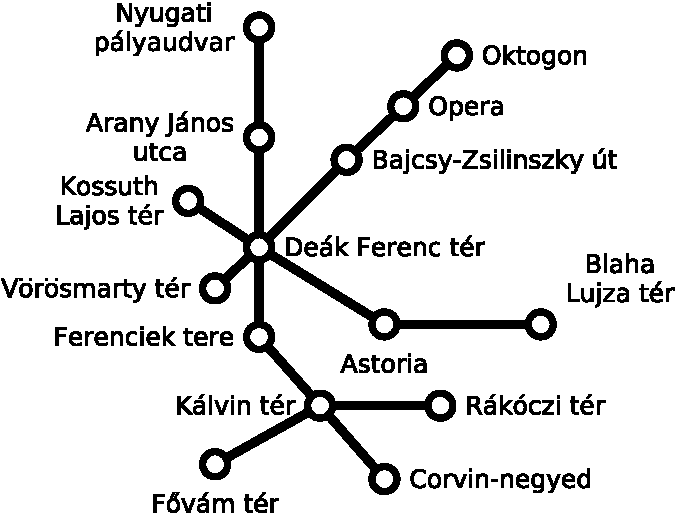
\includegraphics[width=\textwidth]{metrohalozat-nagykorut-egyszeru}
		\caption{A metróhálózat egyszerű gráfként ábrázolva}
		\label{fig:metrohalozat-nagykorut-egyszeru}
	\end{subfigure}
	\caption{Budapest metróhálózata a Nagykörúton belül}\label{fig:animals}
\end{figure}

A modellünk segítségével választ kaphatunk például a következő kérdésekre:

\begin{enumerate}
	\item Milyen megállók érhetők el a Vörösmarty térről indulva?

		Vizsgáljuk meg, hogy a Vörösmarty teret reprezentáló csomópontból kiindulva milyen csomópontok érhetők el. Ehhez elemi gráfbejáró algoritmusok használunk.

		\begin{megjegyzes}
			Elemi útkereső algoritmusok pl. a \roviditesmagyarul{BFS} vagy \roviditesmagyarul{DFS}.
		\end{megjegyzes}
	\item Legalább hány megállót kell utaznunk a Kossuth Lajos tér és a Kálvin tér között?

		A legrövidebb utat szintén kereséssel határozhatjuk meg.

		\begin{megjegyzes}
			Például egy \fogalomragozva{BFS}{szélességi kereséssel}.
		\end{megjegyzes}

\end{enumerate}

Vannak azonban olyan metróközlekedéssel kapcsolatos kérdések, amelyek megválaszolásához a modell nem tartalmaz elég információt:

\begin{enumerate}
	\item Milyen megállók érhetők el a Fővám térről indulva \emph{legfeljebb egy átszállással}?
	\item A menetrend szerint \emph{hány percig tart} az út a Kossuth Lajos tér és az Astoria között?
\end{enumerate}

Ezeknek a kérdéseknek megválaszolásához egészítsük ki a gráfot! Az első kérdéshez szükséges, hogy az egyes metróvonalakat meg tudjuk különböztetni, amit például az élek címkézésével érhetünk el. \Aref{fig:metrohalozat-nagykorut-elcimkezett} ábrán színekkel jelöltük a különböző élcímkéket. Induljunk ki a Fővám térről: átszállás nélkül az Astoria és a Rákóczi tér megállókat érhetjük el, míg egy átszállással elérhetjük az M3-as metró vonalán található megállókat is.

\begin{figure}[H]
	\begin{subfigure}[b]{0.5\textwidth}
		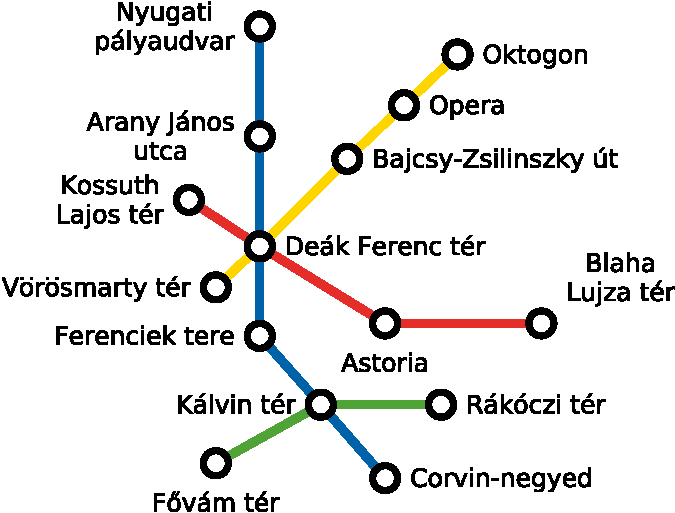
\includegraphics[width=\textwidth]{metrohalozat-nagykorut-elcimkezett}
		\caption{A gráf élcímkékkel kiegészítve}
		\label{fig:metrohalozat-nagykorut-elcimkezett}
	\end{subfigure}
	~
	\begin{subfigure}[b]{0.5\textwidth}
		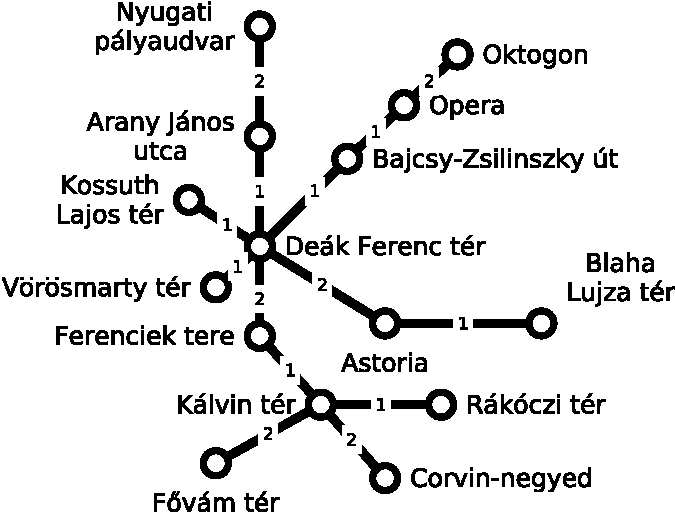
\includegraphics[width=\textwidth]{metrohalozat-nagykorut-elsulyozott}
		\caption{A gráf élsúlyokkal kiegészítve}
		\label{fig:metrohalozat-nagykorut-elsulyozott}
	\end{subfigure}
	\caption{A metróhálózatot ábrázoló gráf kiterjesztései}\label{fig:animals}
\end{figure}

A második kérdés megválaszolásához az egyes megállók közötti utazási időt kell jellemeznünk. Ehhez vegyünk fel \fogalomragozva{elsuly}{élsúlyokat} a gráfba. \Aref{fig:metrohalozat-nagykorut-elsulyozott} ábrán élsúlyokkal jelöltük az egyes megállók között menetidőt. Ezek ismeretében meghatározható a Kossuth Lajos tér és a Kálvin tér közötti út menetrend szerinti időtartama. Ez a modell arra is alkalmas, hogy meghatározzuk a legrövidebb utat a két csomópont között, például a \fogalom{Dijsktra-algoritmus} segítségével.

\begin{pelda}
	Melyik metróvonalak között tudunk átszállni? A kérdésre választ kaphatunk a fenti modell segítségével. Nagyméretű hálózat esetén azonban már sokáig tarthat a válasz meghatározása, ezért érdemes olyan modellt készíteni, ami a válaszhoz nem szükséges részeket \fogalomragozva{absztrakcio}{absztrahálja}.
\end{pelda}

\remofigscale{metro-atszallas}{Átszállási lehetőségek a metróvonalak között a Nagykörúton belül}{\yedscale}

\Aref{fig:metro-atszallas}. ábrán látható modellből azonnal kiderül, hogy mely metróvonalak között van átszállási lehetőség. A modell segítségével tehát hatékonyabban tudunk válaszolni erre a kérdésre, de a korábbi kérdésekhez szükséges információt elvesztettük az absztrakció során.

A közlekedési hálózathoz hasonlóan sok rendszer jól modellezhető gráffal: az élőlények táplálkozási lánca, a közösségi hálók, az úthálózat, telekommunikációs hálózatok stb.

\subsection{Hierarchikus rendszerek}
\label{sec:hierarhcikus-rendszerek}

\begin{pelda}
	Budapestnek 23 kerülete van, amelyek további városrészekből állnak. %\footnote{\url{https://hu.wikipedia.org/wiki/Budapest_v\%C3\%A1rosr\%C3\%A9szeinek_list\%C3\%A1ja}} A metróhálózat megálló különböző városrészekben találhatók.
	Melyik városrészben van az Opera metrómegállója? Melyik városrészben van a legtöbb metrómegálló? Ezekhez hasonló kérdésekre úgy tudunk hatékonyan válaszolni, ha készítünk egy \fogalomragozva{hierarchikus-modell}{hierarchikus modellt} a problémáról.
\end{pelda}

\remofigscale{keruletek-varosreszek-metromegallok}{Budapest kerületei, városrészei és metrómegállói (részleges modell)}{0.5}

Készítsünk modellt, amely ábrázolja Budapest, a kerületek, a városrészek és a metrómegállók viszonyát! \Az+\refstruc{fig:keruletek-varosreszek-metromegallok} modellje négy szintet tartalmaz:

\begin{enumerate}
	\item A hierarchia legfelső szintjén Budapest szerepel.
	\item A második szinten a város kerületei találhatók.
	\item A harmadik szinten az egyes városrészek vannak.
	\item A negyedik szinten a metrómegállók találhatók.
\end{enumerate}

% Érdemes lehetne megemlíteni azt, hogy a kerületek uniója visszaadja Budapestet, a városrészek uniója a kerületeket. Ezzel szemben a metróállomások csak "elemei" a városrészeknek.

Látható, hogy a hierarchikus modellt is ábrázolhatjuk gráfként. A csomópontok a modell különböző szintű elemeit reprezentálják, míg az élek a \fogalomragozva{tartalmazas}{része} viszonyt fejezik ki, például az Opera megálló a VI.~kerület része. A gráf \fogalomragozva{gyoker-csomopont}{gyökér csomópontja} a hierarchiában legmagasabban szereplő elem, Budapest.

Amennyiben egy rendszert hierarchikusan részekre bontunk, nem fordulhat elő, hogy egy elem tartalmazza a szülő elemét, ezért a hierarchikus modelleket reprezentáló gráfok körmentesek. A gyökér elemet leszámítva minden elemnek van szülője, tehát a gráf összefüggő is, így a hierarchikus modellek gráfjai egyúttal \fogalomragozva{fa-graf}{fák}.

\begin{megjegyzes}
	A fa struktúrában a gráf élei \emph{explicit módon} jelölik a tartalmazási hierarchiát. A gyakorlatban nem mindig jelenítjük meg explicit módon a tartalmazási viszonyokat.

	A tartalmazási hierarchia ábrázolható a tartalmazási viszonyok \emph{implicit megjelenítésével} is:

	\begin{figure}[H]
		\centering
		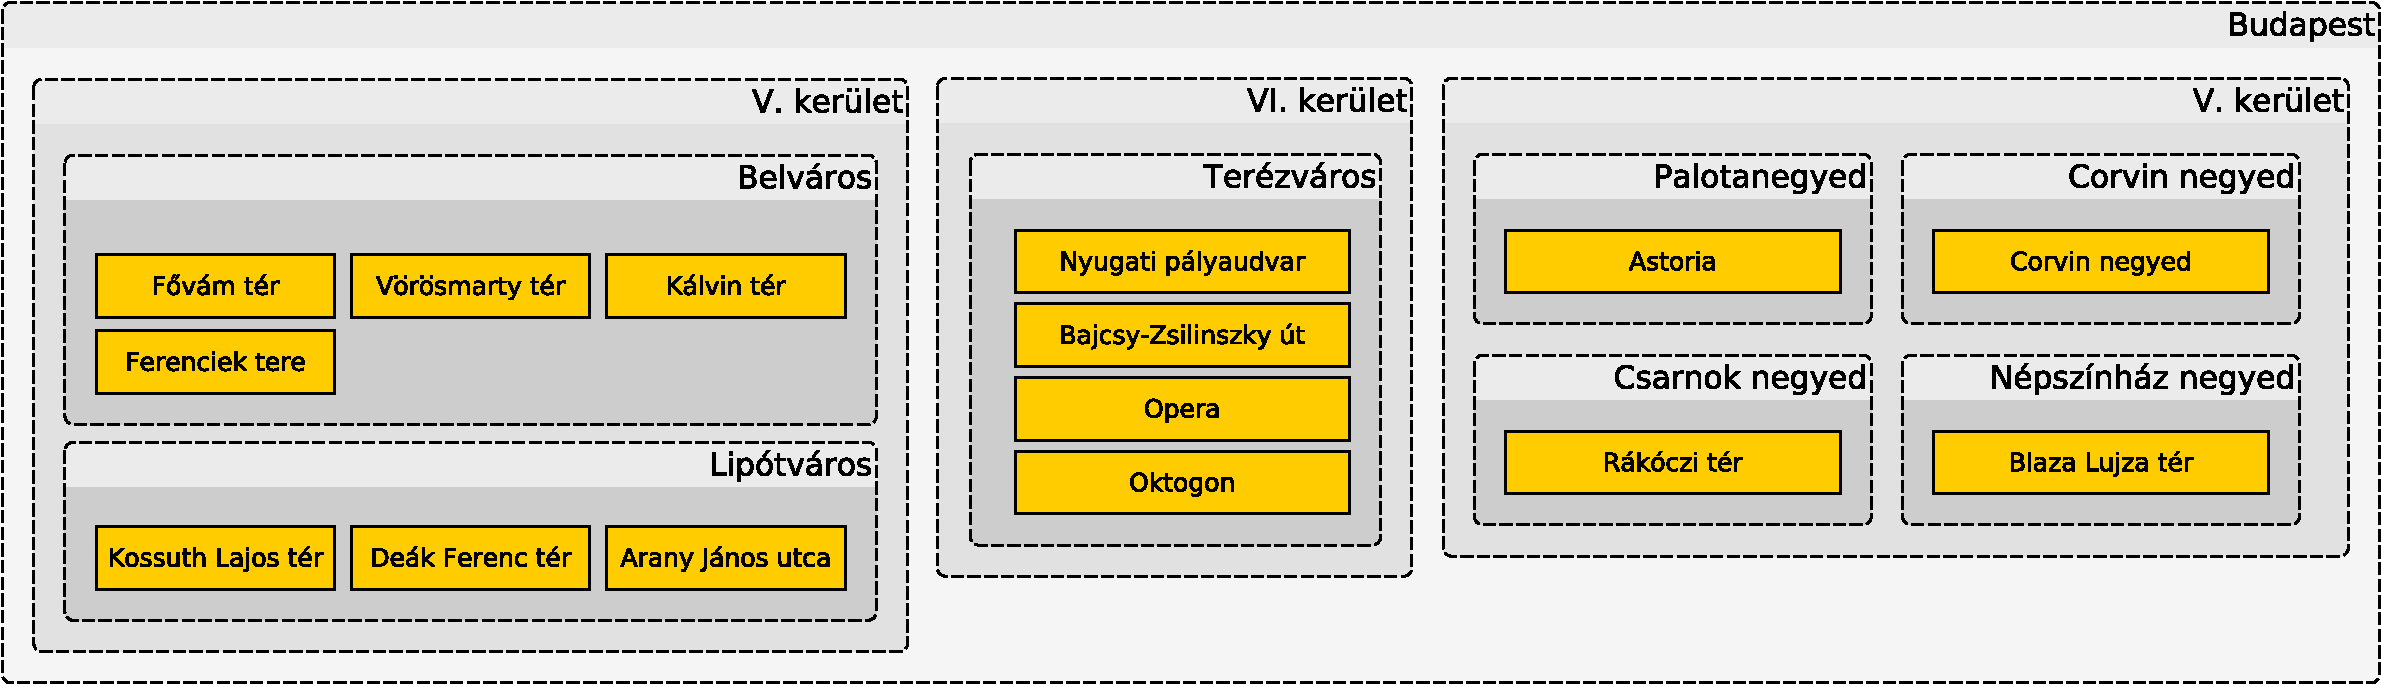
\includegraphics[scale=0.4]{implicit-tartalmazas}
		\caption{A tartalmazási viszonyok implicit módon jelölve}
		\label{fig:implicit-tartalmazas}
	\end{figure}

	\Aref{fig:implicit-tartalmazas}. ábrán egy olyan diagramot látunk, amelyben az egyes síkidomok közötti bennfoglaló ábrázolása reprezentálja a modellben szereplő tartalmazási viszonyt.

%	\added[id=szarnyas]{Ide be is tehetünk egy (kerületeket tartalmazó térképet), az jobb példa az explicit ábrázolásra}
\end{megjegyzes}

Láthattuk tehát, hogy mind a modellelemek közötti kapcsolat, mind a modellhierarchia hatékonyan ábrázolható gráfként. \Aref{fig:metrohalozat-hierarchiaval}. ábrán látható modell \aref{fig:metrohalozat-nagykorut-elcimkezett} és a \ref{fig:keruletek-varosreszek-metromegallok}. ábrákon található metróhálózatot és a területek hierarchiáját is tartalmazza.

\remofigscale{metrohalozat-hierarchiaval}{Budapest metróhálózata és a városrészek, kerületek hierarchiája}{\yedscale}

\subsection{Tulajdonságok}
\label{sec:tulajdonsagok}

\begin{pelda}
A közlekedési vállalat üzemen kívüli járművei telephelyeken parkolnak és itt végzik rajtuk a szükséges karbantartásokat. A metrók telephelyeinek neve metró \emph{járműtelep}, a buszoké az \emph{autóbuszgarázs}.

Mennyi üzemanyag tárolható a legnagyobb autóbusz garázsban? Milyen hosszú a Kőér utcai metró járműtelep vágányhálózata? Ezek a kérdések a modellünk elemeinek tulajdonságaival kapcsolatban merülnek fel. Építsünk modellt a problémára!
\end{pelda}

A telephelyeket például az alábbi modellel írhatjuk le:

\begin{table}[H]
	\centering
	\sf
\centering
\begin{tabular}{rllrrrr}
	\toprule
	\it azonosító & \it helyszín & \it funkció    & \it kapacitás & \it vágányhossz & \it max. üzemanyag &  \\ \midrule
	           T1 & Angyalföld   & kocsiszín      &           147 &          4922 m &                    &  \\
	           T2 & Budafok      & kocsiszín      &            46 &          2750 m &                    &  \\
	           T3 & Cinkota      & autóbuszgarázs &           265 &                 &      250~000 liter &  \\
	           T4 & Kelenföld    & kocsiszín      &            42 &          2829 m &                    &  \\
	           T5 & Kelenföld    & autóbuszgarázs &           322 &                 &      200~000 liter &  \\
	           T6 & Kelenföld    & metró járműterep &           x & yy                &       & \\
	           \bottomrule
\end{tabular}

% https://hu.wikipedia.org/wiki/Kelenf%C3%B6ldi_aut%C3%B3buszgar%C3%A1zs
% http://villamosok.hu/balazs/kcssz/budafok/index.html
% http://kozhir.blog.hu/2012/04/16/vendegsegben_metroeknal
% http://www.ancsingabor.hu/bkv_buszvezeto.html
	\caption{A BKK telephelyei (részleges modell)}
	\label{tab:jarmutelepek}
\end{table}

A modellünk elemei a táblázat sorai. A táblázat fejlécében definiált \fogalomragozva{tulajdonsag}{tulajdonságokból} (pl. helyszín, vágányhossz) az egyes modellelemek eltérő értékeket vehetnek fel. Látható, hogy a táblázatnak nem minden celláját töltöttük ki, mivel az egyes jellemzők nincsenek mindenhol értelmezve.

Megfigyelhetjük azonban, hogy az azonos %\fogalomragozva{tipus}{típussal}
funkcióval rendelkező modellelemek azonos tulajdonságokra vesznek fel értéket.
%Ez alapján megépíthetjük a problémához tartozó \fogalomragozva{tipushierarchia}{típushierarchiát}: minden \textsf{telephely} típusú elemre értelmezzük a helyszín és a kapacitás fogalmakat.
Mindkét típusú telephelynek van \textit{azonosító}, \textit{helyszín}, \textit{funkció} és \textit{kapacitás} attribútuma. Az \textsf{autóbuszgarázs} esetén a \textit{max. üzemanyag}, a \textsf{metró járműtelep} esetében a \textit{vágányhossz} attribútumot rögzítjük.

\subsection{Típusok}

\Aref{tab:jarmutelepek}. táblázatban láthattuk, hogy a \textit{funkció} jellemzővel megkülönböztethetjük az egyes a telephelyeket. Ha a \textit{funkció} jellemzőt a modellelemek \fogalomragozva{tipus}{típusának} tekintjük, akkor úgy is fogalmazhatunk, hogy a \textit{vágányhossz} jellemző csak a \textsf{metró járműtelep} típusú elemekre értelmezett, a \textit{max. üzemanyag} jellemző csak az \textsf{autóbuszgarázs} típusra. A típusokat felhasználhatjuk a gráfok jellemzésére is.

\begin{pelda}
	A korábbi metróhálózatot szeretnénk kiegészíteni a buszhálózatra vonatkozó információval. Szeretnénk tárolni azt is, hogy az egyes vonalakon közlekedő járművek melyik telephelyen parkolnak. Az autóbuszvonalon közelekedő járművek autóbuszgarázsban, a metróvonalon közlekedő járművek metró járműtelepen parkolnak.
\end{pelda}

Készítsünk egy példánygráfot, amelyen ábrázoljuk az M1 és M3-as metróvonal, valamint a 7-es és a 8-as buszvonalak kapcsolódásait (\textit{kapcsolódik) élek}, valamint azt, hogy az egyes vonalak melyik telephelyhez tartoznak (\textit{telephelye) élek}.

\remofigscalefixed{busz-metro-telephelyek}{Közlekedési vonalak és telephelyek}{\yedscale}

A példánygráfot követve a problémához tartozó \fogalomragozva{tipusgraf}{típusgráfban} meg kell jelennie a \textit{vonal} és a \textit{telephely} fogalmaknak. Az egyes vonalak kapcsolódhatnak egymáshoz a \textit{kapcsolódik} él mentén, míg a vonal telephelyét a \textit{telephelye} él jelzi.

\begin{megjegyzes}
Az egyes telephelyek tulajdonságait nem ábrázoltuk az ábrán.
\end{megjegyzes}

\remofigscalefixed{busz-metro-telephelyek-tipusgraf}{Közlekedési vonalak és telephelyek típusgráfja}{\yedscale}

A példánygráfot és a típusgráfot egy gráfban is jelölhetjük. Ekkor az egyes példányok és a típusok között egy \textit{példánya} él fut. % TODO ha az éleknek nincs azonosítójuk, akkor ez élekre nem alkalamzható

\remofigscalefixed{busz-metro-telephelyek-tipusgraffal}{Közlekedési vonalak és telephelyek példány- és típusgráfja}{\yedscale}

\Aref{fig:busz-metro-telephelyek-tipushierarchia}. ábra bemutatja a problémához tartozó \fogalomragozva{tipushierarchia}{típushierarchiát}. A típushierarchia egy hierarchikus modell, amely az egyes típusok leszármazási (\textit{is a}) viszonyait ábrázolja.

\remofigscalefixed{busz-metro-telephelyek-tipushierarchia}{Közlekedési vonalak és telephelyek típushierarchiája}{\yedscale}

A rendszer fejlesztésekor gyakran fontos, hogy a típusgráfot és a típushierarchiát együtt lássuk. A \fogalom{metamodell} tartalmazza a típusgráfot, a típusok hierarchiáját, a tulajdonságmodellt (ill. további, itt nem részletezett szabályokat, pl. multiplicitási kényszerek, jólformáltsági kényszerek). % TODO a legtöbb metamodell nem támogatja az éltípusok öröklési hierarchiáját sem, ezt tipikusan template-ekkel oldják meg

A típusgráfban és a típushierarchiában tartalmazott információt, valamint tulajdonságmodellt együtt modellezve megkapjuk a terület metamodelljét. A metamodell részlete \aref{fig:busz-metro-telephelyek-metamodell}. ábrán látható. Bár az ábrán a csomópontok elrendezése alapján következtethetünk arra, hogy melyik vonalakat látjuk, ezt az információt elvesztettük: ebben a reprezentációban az egyes metróvonalakat nem tudjuk megkülönböztetni.

\remofigscalefixed{busz-metro-telephelyek-metamodell}{Közlekedési vonalak és telephelyek (részleges) metamodellje}{\yedscale}

A példánymodellt és a metamodellt ábrázolhatjuk egyszerre is, a két modell elemei között a \emph{példánya} viszony teremt kapcsolatot (szürke szaggatott nyíl).

\remofigscalefixed{busz-metro-telephelyek-peldanymodell-metamodell}{Közlekedési vonalak és telephelyek példánymodellje és (részleges) metamodellje egy gráfon ábrázolva}{\yedscale}


\begin{feladat}
	Az egyes járműtelepek is valamelyik városrészhez tartoznak. Készítsünk olyan metamodellt, amelyben ábrázolható az egyes járműtelepek és városrészek kapcsolata is!
\end{feladat}



%Felismerhetjük, hogy a telephely helyszíne is belepasszol a városrészes gráfba. Ezzel sok fogalmat elég jól lehet szemléltetni: derived feature-ök, derived referenciák stb.

%\remofigscalefixed{jarmutelepek}{A közlekedési hálózatunk metamodellje}{\yedscale}


%TODO \fogalom{szarmaztatott-tulajdonsag}


%\begin{megjegyzes}
%A Zách utcai trolitelepen buszokat és trolikat is tárolnak. Alakítsuk át a modellt úgy, hogy ezt is tudja modellezni. % http://www.bkk.hu/2013/09/villamosnap-budafokon-es-nyilt-nap-a-trolitelepen/
%\end{megjegyzes}

%\begin{pelda}
%	Melyik a legnagyobb teljesítményű jármű? Milyen jellemzőket kell rögzíteni egy újonnan beszerzett buszról? Ezek a kérdések a modellünk elemeinek tulajdonságaival kapcsolatban merülnek fel.
%\end{pelda}
%
%Készítsünk egy modellt, ami a különböző járműveket tartalmazza. Ezt a modellt gráf helyett inkább táblázatos formában érdemes ábrázolni, így jobban áttekinthető lesz.
%
%\begin{table}[H]
%	\centering
%	\begin{tabular}{|l|l|l|l|l|r|l|l|}
%		\hline
%		név                   & típus    & tömeg & hossz & lökettérfogat & \#motorok & telj. & nyomtáv \\ \hline\hline
%		Volvo 7700            & busz     & 18 t  & 12 m  & 9000 cm$^3$   &               & 320 LE       &         \\ \hline
%		Siemens Combino Supra & villamos & 70 t  & 54 m  &               & 8             & 800 kW       & 1800 mm \\ \hline
%		XY & villamos & a t  & b m  &               & 8             & yy kW       & 1800 mm \\ \hline
%		Alstom Metropolis     & metró    &       &       &               &               &              & 1435 mm \\ \hline
%	\end{tabular}
%	\caption{Járművek tulajdonságai}
%	\label{tab:jarmuvek}
%\end{table}
%
%A modellünk elemei itt a táblázat sorai. A modellelemek tulajdonságait \fogalomragozva{jellemzo}{jellemzőkkel} vagy más néven \fogalomragozva{attributum}{attribútumokkal} írjuk le. Mint \aref{tab:jarmuvek}. táblázatban látható, különböző modellelemekre az egyes jellemzők más-más értéket vehetnek fel. Látható, hogy a táblázatnak nem minden celláját töltöttük ki, mivel az egyes jellemzők nincsenek mindenhol értelmezve. Ezeket a cellákat gyakran az \rovidites{NA} (\roviditesangolul{NA}) rövidítéssel vagy \textsf{null} értékkel jellemezzük. Megfigyelhetjük azonban, hogy az azonos \fogalomragozva{tipus}{típussal} rendelkező modellelemek azonos tulajdonságokra vesznek fel értéket.

%A jellemzők nem is feltétlenül értelmezettek minden modellelemre (ún. \fogalomragozva{parcialis-fuggveny}{parciális függvényként} írhatóak le a matematika nyelvén).


%%%%%%%%%%%%%%%%%%%%%%%%%%%%%%%%%%%%%%%%%%%%%%%%%%%%%%%%%%%%%%%%%%%%%%%%%%%%%%%%

\section{A strukturális modellezés elmélete}

%Ahogy \az+\refstruc{sec:motivacio}

Ahogy az eddigi példákban láttuk, a strukturális modellezés célja, hogy a rendszer felépítését jellemezze, beleértve az egyes elemek típusát, a közöttük lévő kapcsolatokat és hierarchiát, valamint az elemek tulajdonságait. Egy rendszer strukturális modellje tehát alkalmas arra, hogy az alábbi kérdésekre (nem feltétlenül kimerítő) választ nyújtson:

\begin{itemize}
	\item Milyen elemekből áll a rendszer?
	\item Hogyan kapcsolódnak egymáshoz az elemek?
	\item Milyen hierarchia szerint épül fel a rendszer?
	\item Milyen tulajdonságúak a rendszer elemei?
\end{itemize}

%A strukturális modell elkészítéséhez jellemeznünk kell a rendszerünk elemeinek aspektusait: a típusukat, az elemek közötti hierarchiát és kapcsolatokat, valamint az elemek jellemzőit.

A strukturális modellre az alábbi tömör definíciót adhatjuk.

\begin{definicio}
	A \fogalom{strukturalis-modell} a rendszer felépítésére (\fogalomragozva{struktura}{struktúrájára}) vonatkozó tudás. A strukturális modell a rendszer alkotórészeire, ezek tulajdonságaira és egymással való viszonyaira vonatkozó statikus (tehát változást nem leíró) tudást reprezentál. %Az egyes modellelemek \fogalomragozva{egyedi}{egyediek}.
\end{definicio}

\begin{megjegyzes}
Fontos, hogy maga a strukturális modell változhat az idő során (pl. a metróhálózat fejlődik), de maga a modell nem ír le időbeli változásokat (pl. hogy miként mozognak a szerelvények).
\end{megjegyzes}

%A strukturális modell aspektusa: fizikai (felépítés), logikai (funkció)

A következőkben a korábbi példákra építve bemutatjuk a strukturális modellezés elméleti hátterét és precízen definiáljuk a szükséges fogalmakat.

\subsection{Tulajdonságmodell}

\begin{definicio}
	A \fogalom{jellemzo} egy, a modell által megadott \fogalom{parcialis-fuggveny}, amelyet a modellelemeken értelmezünk.
\end{definicio}

\begin{megjegyzes}
	A $H$ halmazon értelmezett \fogalom{parcialis-fuggveny} nem jelent mást, mint a $H$ valamely (nem megnevezett) részhalmazán értelmezett \fogalom{fuggveny}. Konkrét esetünkben az egyes jellemzőket a modellelemek egy-egy részére értelmezzük (nem feltétlenül az összesre).
\end{megjegyzes}

A jellemzőket gyakran táblázatos formában ábrázoljuk. Vizsgáljuk meg például \aref{tab:jarmutelepek}. táblázat jellemzőit:

\begin{table}[H]
	\centering
	\sf
\centering
\begin{tabular}{rllrrrr}
	\toprule
	\it azonosító & \it helyszín & \it funkció    & \it kapacitás & \it vágányhossz & \it max. üzemanyag &  \\ \midrule
	           T1 & Angyalföld   & kocsiszín      &           147 &          4922 m &                    &  \\
	           T2 & Budafok      & kocsiszín      &            46 &          2750 m &                    &  \\
	           T3 & Cinkota      & autóbuszgarázs &           265 &                 &      250~000 liter &  \\
	           T4 & Kelenföld    & kocsiszín      &            42 &          2829 m &                    &  \\
	           T5 & Kelenföld    & autóbuszgarázs &           322 &                 &      200~000 liter &  \\
	           T6 & Kelenföld    & metró járműterep &           x & yy                &       & \\
	           \bottomrule
\end{tabular}

% https://hu.wikipedia.org/wiki/Kelenf%C3%B6ldi_aut%C3%B3buszgar%C3%A1zs
% http://villamosok.hu/balazs/kcssz/budafok/index.html
% http://kozhir.blog.hu/2012/04/16/vendegsegben_metroeknal
% http://www.ancsingabor.hu/bkv_buszvezeto.html
\end{table}


\begin{megjegyzes}
	A tulajdonságmodell mögötti matematikai struktúra az ún. \fogalomragozva{relacio}{reláció}. A reláció pontos halmazelméleti definíciójával és a relációkon értelmezett műveleteket definiáló \fogalomragozva{relacioalgebra}{relációalgebrával} bővebben az \adatb tárgy foglalkozik.
\end{megjegyzes}

A modellelemeket az \textit{azonosító} jellemzőjükkel különböztetjük meg egymástól. % rendelkeznek \fogalomragozva{egyedi-azonosito}{egyedi azonosítóval}.
A \textit{kapacitás} jellemzőhöz tartozó függvény
$\mathit{kapacitás}(e) \rightarrow n,$
ahol $e$ egy modellelem azonosítója, $n$ egy nemnegatív egész szám.
Például
$$\mathit{kapacitás}(\mathsf{T2}) = 60, \quad \mathit{kapacitás}(\mathsf{T3}) = 265.$$

A \textit{funkció} jellemzőhöz tartozó függvény
$\mathit{funkció}(e) \rightarrow t,$
ahol $e$ egy modellelem azonosítója, $t$ a $\{\textsf{metró járműtelep}, \textsf{autóbuszgarázs}\}$ halmaz eleme.
Például
$$\mathit{funkció}(\mathsf{T2}) = \textsf{metró járműtelep}, \quad \mathit{funkció}(\mathsf{T3}) = \textsf{autóbuszgarázs}.$$

A fentiekhez hasonlóan, a \textit{vagányhossz} jellemzőhöz tartozó parciális függvény
$\mathit{vagányhossz}(e) \rightarrow n,$
ahol $e$ egy modellelem azonosítója, $n$ egy nemnegatív egész szám. Fontos különbség viszont az eddigiekhez képest, hogy ezt jellemzőt csak bizonyos modellelemekre értelmeztünk, másokra nem: a metró járműtelepek esetén vesz fel értéket, az autóbuszgarázsok esetén viszont nem. Vagyis látható, hogy a \textit{vagányhossz} jellemző csak akkor vesz fel értéket, ha a \textit{funkció} attribútum értéke \textsf{metró járműtelep}.

Ha tehát a \textit{funkció} attribútumot a telephely \fogalomragozva{tipus}{típusának} tekintjük, akkor úgy is fogalmazhatunk, hogy a \textit{vágányhossz} jellemző csak a \textsf{metró járműtelep} típusú elemekre értelmezett. Általánosan:

\begin{definicio}
	A \fogalom{tipus} egy kitüntetett jellemző, amely meghatározza, hogy milyen más jellemzők lehetnek értelmezettek az adott modellelemre, illetve milyen más modellelemekkel lehet kapcsolatban. A többi jellemzőt \fogalomragozva{tulajdonsag}{tulajdonságnak} hívjuk.

\begin{megjegyzes}
	Jelen anyagban az egyszerűség kedvéért feltételezzük, hogy a modellelemeknek pontosan egy típusa van.
\end{megjegyzes}
\end{definicio}


A modellünkben két típus van: az \textsf{autóbuszgarázs} és a \textsf{járműtelep}. Például a cinkotai telephely az \textsf{autóbuszgarázs}, míg a mexikói úti telephely a \textsf{metró járműtelep} típus példánya.

\begin{definicio}
Egy adott $t$ típus \fogalomragozva{peldany}{példányainak} nevezzük azon modellelemeket, amelyek típusa $t$.
\end{definicio}

A modellezési gyakorlatban elterjedt (de nem univerzális) megkötés, hogy az egyes elemek típusát állandónak tekintjük. Ha az elem típusa a rendszer működése során nem változhat meg, akkor olyan típust kell hozzárendelni, amely az elem teljes életciklusa során előforduló összes lehetséges jellemzővel, kapcsolattal összhangban van.

\subsection{Gráfmodellek}

\begin{kisdefiniciok}
	A definíciók támaszkodnak a gráfelmélet alapjaira, ezért röviden összefoglaljuk a felhasznált definíciókat.

	A \fogalom{graf} egy olyan $G = (V, E)$ struktúra, ahol $V$ halmaz a csomópontok, $E$ az élek halmaza. Az élek csomópontok között futnak, \fogalom{iranyitatlan-graf} esetén az $E$ halmaz csomópontok rendezetlen $\{v_1, v_2\}$ párjaiból áll (tehát nem különböztetjük meg a $\{v_1, v_2\}$ és a $\{v_2, v_1\}$) párokat, míg \fogalom{iranyitott-graf} esetén csomópontok rendezett $(v_1, v_2)$ párjaiból.
	% Egy gráf \fogalomragozva{egyszeru-graf}{egyszerű}, ha nem tartalmaz többszörös és hurokélet.

	\fogalomragozva{cimkezett-graf}{Címkézett gráf} esetén a gráf elemeit (csomópontjait és/vagy éleit) \fogalomragozva{cimke}{címkékkel} láthatjuk el. A címkézés célja lehet \fogalom{egyedi-azonosito} hozzárendelése vagy bizonyos tulajdonság leírása (pl. a csomópontok kapacitása, élek típusa). Ha precízen szeretnénk jellemezni a gráfot, a következő terminológiát használhatjuk: ha csak a csomópontokhoz rendelünk címkéket, \fogalomragozva{csucscimkezett-graf}{csúcscímkézett} gráfról beszélünk, míg ha csak a gráf éleihez rendelünk címkéket, \fogalomragozva{elcimkezett-graf}{élcímkézett} gráfról beszélünk.

	%A \fogalom{sulyozott-graf} olyan $(G, w)$ pár, ahol $G = (V, E)$ gráf, $w: E \rightarrow \mathbb{R}$ egy súlyfüggvény.
\end{kisdefiniciok}

A típusok gráf jellegű modellek esetén is fontos szerepet játszanak. A gráfmodell elemeit (külön-külön a csomópontokat és az éleket is) típusokba sorolhatjuk. A típusok meghatározzák, hogy az egyes csomópontok milyen élekkel köthetők össze.

Az egyes csomópont- és éltípusok viszonyát gráfként is ábrázolhatjuk.

\begin{definicio}
	A \fogalom{tipusgraf} egy olyan gráf, amelyben minden csomóponttípushoz egy típuscsomópont, minden éltípushoz egy típusél tartozik.
\end{definicio}

A gráfmodelleken is értelmezzük a \fogalom{peldany} fogalmát.

\begin{definicio}
	Egy adott típusgráf \fogalomragozva{peldanygraf}{példánygráfja} alatt olyan gráfmodellt értünk, amelynek elemei a típusgráf csomópont- és éltípusainak példányai, valamint minden él forrása és célja rendre az éltípus forrásának és céljának példánya.
\end{definicio}

A típusgráfot és példánygráfot egy gráfon ábrázolva a típus-példány viszonyok is megjeleníthetők: a példánygráf csomópontjaiból a típusgráf csomópontjaira \fogalomangolul{peldanya} (\fogalom{peldanya}) élek mutatnak. Szintén \fogalomangolul{peldanya} viszony áll fenn a példánygráf élei és a típusgráf élei között.% -- ennek ábrázolása azonban gráfként nehézkes.

\begin{megjegyzes}
	Az \fogalomangolul{peldanya} viszony helyett gyakran annak inverzét, a \fogalomangolul{tipusa} (x \fogalom{tipusa} y-nak) viszonyt. Gráfban ábrázolva az \fogalom{peldanya} és \fogalom{tipusa} élek adott csomópontok között egymással ellentétes irányúak.
\end{megjegyzes}

\remofigscalefixed{busz-metro-telephelyek-tipusgraf-inverz-elek}{Példány és típusgráf \fogalomangolul{tipusa} élekkel}{\yedscale}

\begin{definicio}
	Egy rendszer \fogalomragozva{metamodell}{metamodellje} tartalmazza a típusgráfot, az egyes típusok közötti kapcsolatokat, ill. további megkötéseket is.

	\begin{megjegyzes}
		A további megkötések között szerepelhetnek jólformáltsági kényszerek, multiplicitási kényszerek stb. Ezekkel most nem foglalkozunk részletesen.
	\end{megjegyzes}
\end{definicio}

\subsection{Hierarchia}

\begin{kisdefiniciok}
	A \fogalom{seta} szomszédos csúcsok és élek váltakozó sorozata, mely csúccsal kezdődik és csúcsban végződik. %Ha egy séta során egy gráfelemet sem érintünk többször, útról beszélünk, tehát
	Az \fogalom{ut} olyan séta, amely nem metszi önmagát, valamint első és utolsó csúcsa különbözik. A \fogalom{kor} olyan séta, amely nem metszi önmagát, valamint első és utolsó csúcsa megegyezik. %Körről beszélünk, ha egy út során ugyanoda érünk vissza, ahonnan elindultunk.
	%Ezek ismeretében már beszélhetünk körmentes gráfokról.
	A körmentes, összefüggő gráfokat \fogalomragozva{fa-graf}{fának} nevezzük. (A körmentes gráfokat \fogalomragozva{erdo}{erdőnek} nevezzük.)
	A fák esetén gyakran kiemelt szerepet tulajdonítunk egy csomópontnak: a \fogalom{gyoker-csomopont} a fa egy megkülönböztetett csomópontja. A \fogalom{gyokeres-fa} olyan fa, ami rendelkezik gyökér csomóponttal. \Fogalom{gyokeres-szintezett-fa} esetén a fa csomópontjaihoz hozzárendeljük a gyökértől vett távolságukat is.

	A hierarchikus modellezésben kiemelt szerepet játszanak az irányított körmentes gráfok. Egy gráf \rovidites{DAG} (\roviditesangolul{DAG}), ha nem tartalmaz irányított kört.
\end{kisdefiniciok}

Egy rendszer hierarchiája a rendszer dekompozíciójával állítható elő.

\begin{definicio}
	A \fogalom{dekompozicio} (\fogalom{faktoring}) egy rendszer kisebb \fogalomragozva{komponens}{komponensekre} bontása, amelyek könnyebben érthetők, fejleszthetők és karbantarthatók.
\end{definicio}

A rendszer így kapott egyes komponensei (részrendszerei) gyakran további dekompozícióval még kisebb részekre bonthatóak. Természetesen a dekompozíció során ügyelnünk kell arra, hogy az egyes részekből visszaállítható legyen az eredeti rendszer, különben a kapott strukturális modellünk hiányos.

\begin{definicio}
	Egy dekompozíció \fogalomragozva{helyes-dekompozicio}{helyes}, ha a dekompozícióval kapott rendszer minden elemének megfeleltethető az eredeti rendszer valamelyik eleme, és az eredeti rendszer minden eleméhez hozzárendelhető a dekompozícióval kapott rendszer egy vagy több eleme.
\end{definicio}


%Korábban láttuk, hogy a hierarchiában nincs kör és ezt egyébként fának nevezzük. Ha irányított a gráf, akkor az a fontos, hogy irányított kör ne legyen benne.

%A hierarchiát reprezentáló modellek körmentes gráfot alkotnak, szigorú hierarchia esetén ez \fogalomragozva{fa-graf}{fa} vagy \fogalom{erdo}, megengedő hierarchia esetén \rovidites{DAG}.










%%%%%%%%%%%%%%%%%%%%%%%%%%%%%%%%%%%%%%%%%%%%%%%%%%%%%%%%%%%%%%%%%%%%%%%%%%%%%%%%%%%%%%%%%%%%%%%%%%%%



\section{Nézetek}

A struktúramodellekből különböző \fogalomragozva{nezet}{nézeteket} állíthatunk elő.

Tulajdonságmodelleken a leggyakrabban használt műveletek a \fogalom{szures} és a \fogalom{vetites}. Ezek során úgy \fogalomragozva{absztrakcio}{absztraháljuk} a modellt, hogy bizonyos modellelemeket és/vagy azok egyes jellemzőit elhagyjuk.

\begin{megjegyzes}
	A relációalgebrában a \fogalom{szures} művelet neve \fogalom{szelekcio}, a \fogalom{vetites} művelet neve \fogalom{projekcio}.
\end{megjegyzes}

\subsection{Szűrt nézet}

Ismét idézzük fel \az+\refstruc{tab:jarmutelepek} telephelyeket tartalmazó tulajdonságmodelljét.

\begin{table}[H]
	\centering
	\sf
\centering
\begin{tabular}{rllrrrr}
	\toprule
	\it azonosító & \it helyszín & \it funkció    & \it kapacitás & \it vágányhossz & \it max. üzemanyag &  \\ \midrule
	           T1 & Angyalföld   & kocsiszín      &           147 &          4922 m &                    &  \\
	           T2 & Budafok      & kocsiszín      &            46 &          2750 m &                    &  \\
	           T3 & Cinkota      & autóbuszgarázs &           265 &                 &      250~000 liter &  \\
	           T4 & Kelenföld    & kocsiszín      &            42 &          2829 m &                    &  \\
	           T5 & Kelenföld    & autóbuszgarázs &           322 &                 &      200~000 liter &  \\
	           T6 & Kelenföld    & metró járműterep &           x & yy                &       & \\
	           \bottomrule
\end{tabular}

% https://hu.wikipedia.org/wiki/Kelenf%C3%B6ldi_aut%C3%B3buszgar%C3%A1zs
% http://villamosok.hu/balazs/kcssz/budafok/index.html
% http://kozhir.blog.hu/2012/04/16/vendegsegben_metroeknal
% http://www.ancsingabor.hu/bkv_buszvezeto.html
\end{table}

\begin{definicio}
	A \fogalomragozva{szures}{szűrés} művelet során a modell elemein kiértékelünk egy feltételt és azokat tartjuk meg, amelyek megfelelnek a feltételnek.
\end{definicio}

Tulajdonságmodellek esetén a szűrés az elhagyott modellelemek a modell sorai lehetnek, gráf jellegű modellek esetén a gráf csúcsai vagy élei.

\subsubsection{Tulajdonságmodell szűrése}

\begin{pelda}
	Szeretnénk megtudni, hogy mely telephely alkalmas legalább 100 jármű befogására.
\end{pelda}

Azokra az elemekre szűrünk, amelyeknél a \textsf{kapacitás} jellemző értéke 100-nál nagyobb vagy egyenlő.
%$$\sigma_{\mathsf{kapacitás} \,\geq\, 100} (\textsf{telephely})$$

Az eredmény:
\begin{table}[H]
	\centering
	\sf
	\centering
	\begin{tabular}{rllrrrr}
		\toprule
		\it azonosító & \it helyszín & \it funkció      & \it kapacitás & \it vágányhossz & \it max. üzemanyag &  \\ \midrule
		T3 & Cinkota      & autóbuszgarázs   &           265 &                 &      250~000 liter &  \\
		T4 & Kelenföld    & autóbuszgarázs   &           322 &                 &      200~000 liter &  \\
		\bottomrule
	\end{tabular}
\end{table}

\begin{pelda}
	Szeretnénk megtudni, hogy mely metró járműtelep alkalmas legalább 50 jármű befogására.
\end{pelda}

Végezzünk szűrést azokra a modellelemekre, ahol a \textit{funkció} attribútum értéke \textsf{metró járműtelep}, a \textit{kapacitás} attribútum értéke nagyobb vagy egyenlő 50-nél.

Az eredmény:
\begin{table}[H]
	\sf
	\centering
	\begin{tabular}{rllrrrr}
		\toprule
		\it azonosító & \it helyszín & \it funkció      & \it kapacitás & \it vágányhossz & \it max. üzemanyag &  \\ \midrule
		T2 & Kőér utcai   & metró járműtelep &            60 &        16~512 m &                    &  \\
		\bottomrule
	\end{tabular}
\end{table}

\subsubsection{Gráfmodell szűrése}

Egy gráfmodellből a szűrés a modell egy \fogalomragozva{reszgraf}{részgráfját} állítja elő.

\begin{pelda}
	Soroljuk fel az M2-es és az M4-es metró megállóit.
\end{pelda}

A modellen szűrést végzünk, ami csak azokat a csomópontokat tartja meg, amelyekhez tartozik olyan él, amelynek a címkéje M2 vagy M4. A kapott részgráf \aref{fig:metrohalozat-nagykorut-elcimkezett-szurt} ábrán látható.

\begin{pelda}
	Határozzuk meg, hogy mely szomszédos metrómegállók között hosszabb egy percnél a menetidő.
\end{pelda}

A modellen szűrést végzünk, ami

\begin{itemize}
	\item csak azokat a csomópontokat tartja meg, amelyekhez tartozik 1-nél nagyobb súlyú él,
	\item csak az 1-nél nagyobb súlyú éleket tartja meg.
\end{itemize}

A kapott részgráf \aref{fig:metrohalozat-nagykorut-elsulyozott-szurt} ábrán látható.

\begin{figure}[H]
	\begin{subfigure}[b]{0.5\textwidth}
		\centering
		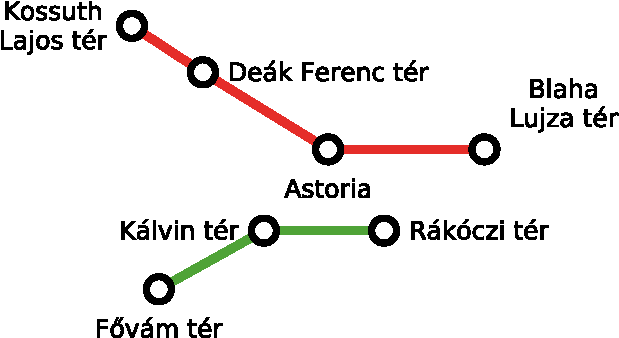
\includegraphics[scale=\yedscale]{metrohalozat-nagykorut-elcimkezett-szurt}
		\caption{Az M2 és az M4 metróvonalak megállói}
		\label{fig:metrohalozat-nagykorut-elcimkezett-szurt}
	\end{subfigure}
	~
	\begin{subfigure}[b]{0.5\textwidth}
		\centering
		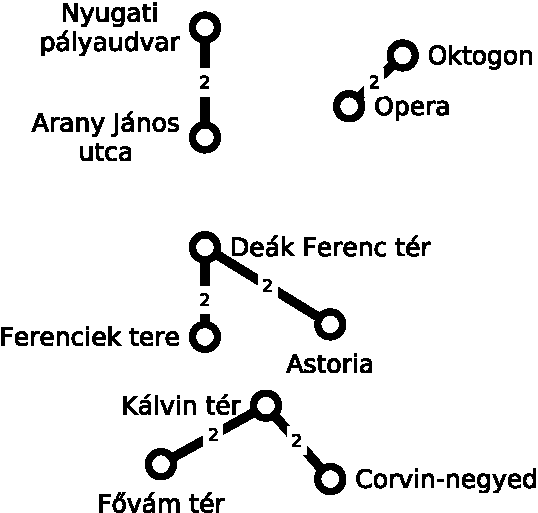
\includegraphics[scale=\yedscale]{metrohalozat-nagykorut-elsulyozott-szurt}
		\caption{Az 1 percnél távolabbi metrómegállók}
		\label{fig:metrohalozat-nagykorut-elsulyozott-szurt}
	\end{subfigure}
	\caption{Szűrések a metróhálózatot tartalmazó gráfon}
\end{figure}


\subsection{Vetített nézet}

\begin{definicio}
	\Fogalom{vetites} során a modell egyes jellemzőit kiválasztjuk és a többit elhagyjuk a táblázatból.

\begin{megjegyzes}
	Érvényes vetítés művelet az is, ha a tulajdonságmodell összes jellemzőjét megtartjuk.
\end{megjegyzes}
\end{definicio}

\subsubsection{Tulajdonságmodell vetítése}

\begin{pelda}
	Olyan kimutatásra van szükségünk, ami csak az egyes telephelyek helyszínét, funkcióját és kapacitását tartalmazza.
%	$$\pi_{\textsf{helyszín, kapacitás}} (\textsf{telephely})$$
\end{pelda}

Végezzünk szűrést a tulajdonságmodelleken a \textit{helyszín}, \textit{funkció} és a \textit{kapacitás} attribútumokra.

\begin{table}[H]
	\sf
	\centering
	\begin{tabular}{llr}
		\toprule
		\it helyszín & \it funkció      & \it kapacitás \\ \midrule
		Mexikói út   & metró járműtelep &            24 \\
		Kőér utcai   & metró járműtelep &            60 \\
		Cinkota      & autóbuszgarázs   &           265 \\
		Kelenföld    & autóbuszgarázs   &           322 \\ \bottomrule
	\end{tabular}
\end{table}

%\subsubsection{Gráfmodell vetítése}
%
%A tulajdonságmodellhez hasonlóan a gráfmodellből is elhagyhatunk jellemzőket.
%
%\begin{pelda}
%	\ldots
%\end{pelda}
%
%\ldots

%%%%%%%%%%%%%%%%%%%%%%%%%%%%%%%%%%%%%%%%%%%%%%%%%%%%%%%%%%%%%%%%%%%%%%%%%%%%%%%%%%%%%%%%%%%%%%%%%%%%

\section{Strukturális modellezési technikák}

%Fontos gondolat: a strukturális modellezésnek többféle célja lehet.
%
%
%\begin{itemize}
%	\item Készítsünk egy adatmodellt a rendszerünkhöz, pl. egy pizzarendelő oldalon elkészítjük az adatbázis modelljét. Ezután az adatbázis a felhasználói interakcióknak megfelelően változik. Ez a modell ,,típusgráf'' része.
%
%	\item Készítsünk a problémából egy modellt, amiből bizonyos kérdésekre választ kaphatunk. Például az alaprajzával modellezzünk egy épületet és nézzük meg, hogy bizonyos tűzvédelmi szempontoknak megfelel-e. Ez a modell ,,példánygráf'' része.
%\end{itemize}

A modellezési formalizmusok után bemutatunk néhány strukturális modellezési technikát.

\subsection{Hierarchia modellezése}

Korábban láttuk, hogy a modellelemek közti szigorú hierarchia kifejezhető fa (ill. erdő) gráfokkal. Ezek a fajta modellek képesek kifejezni a (rész)rendszerek és alkotóelemeik közti tartalmazási viszonyt, akár többszintű tartalmazással is (a részrendszerek is további részeket tartalmaznak). Azonban a gyakorlatban a modellnek sokszor ennél jóval több információt kell tartalmaznia; egy-egy adott modellelemmel kapcsolatban nem csak a tartalmazó és tartalmazott komponenseivel való tartalmazási viszonyát kell ismerni, hanem egyéb modellelemekkel való kapcsolatait.

Ilyenkor a strukturális modell (gráf jellegű része) két rétegre tagozódik: egyrészt a modell szerkezeti vázát alkotó tartalmazási hierarchiára (fa/erdő), amely az alkotóelemek rész-egész viszonyait reprezentálja, másrészt ezen felüli \fogalom{kereszthivatkozas} élekre, amelyek a tartalmazási rendtől függetlenül, a körmentesség korlátozása nélkül köthetnek össze elemeket. Ennek megfelelően egy metamodell megmondhatja, hogy mely éltípusok példányait fogjuk az említett szerkezeti vázat alkotó tartalmazási éleknek tekinteni.

A hierarchikus modellek megalkotása, illetve az összetett rendszerek tervezése során többféleképp választható meg az egyes elemek elkészítésének sorrendje. Jól illusztrálja a választási szabadságot két polárisan ellentétes megközelítés: a \fogalomangolul{top-down} és a \fogalomangolul{bottom-up} modellezés.

\begin{definicio}
	\Fogalomangolul{top-down} modellezés során a rendszert felülről lefelé (összetett rendszerből az alkotóelemei felé haladva) építjük. A modellezés alaplépése a \fogalom{dekompozicio}.
\end{definicio}

Egy top-down modellezési / tervezési folyamatot úgy kell tehát elképzelni, hogy a kezdetektől fogva az egész rendszer modelljét építjük; azonban eleinte hiányoznak még a részletek. Idővel a modellt finomítjuk: tartalmazott alkotóelemekre bontjuk a rendszert, megadva azok tulajdonságait és kereszthivatkozásait is; majd később magukat az alkotóelemeket ugyanúgy strukturális dekompozíciónak vetjük alá.

A top-down modellezés fontos jellemzői:

\begin{itemize}
	\item[$\oplus$] Részrendszer tervezésekor a szerepe már ismert
	\item[$\ominus$] ,,Félidőben'' még nincsenek működő (teljes részletességgel elkészített) részek
	\item[$\ominus$] Részek problémái, igényei későn derülnek ki
\end{itemize}

\begin{definicio}
	\Fogalomangolul{bottom-up} modellezés során a rendszert alulról felfelé (elszigetelt alkotóelemekből az összetett rendszer felé haladva) építjük. A modellezés alaplépése a \fogalom{kompozicio}: az egész rendszer összeszerkesztése külön modellezett vagy fejlesztett részrendszerekből.
\end{definicio}

Egy bottom-up modellezési / tervezési folyamatot úgy kell tehát elképzelni, hogy a kezdetektől fogva részletes modelleket építünk; azonban eleinte csak a rendszer izolált, egyszerű komponenseivel foglalkozunk. Ahogy fokozatosan egyre több komponens készül el, nagyobb részrendszerekké foglalhatjuk őket össze, az egymáshoz való kapcsolódásukat is tisztázva. Idővel az így kapott összetettebb részrendszereket is további kompozíciónak vethetjük alá.

A bottom-up modellezés fontos jellemzői:

\begin{itemize}
	\item[$\oplus$] A rendszer részei önmagukban kipróbálhatók, tesztelhetők
	\item[$\oplus$] Részleges készültségnél könnyebben előállítható a rendszer prototípusa
	\item[$\ominus$] Nem látszik előre a rész szerepe az egészben
\end{itemize}

Természetesen a gyakorlatban a kétféle szélsőséges megközelítés közti kompromisszum is elképzelhető.

%\subsection{Metamodellezés}
%
%Egy adott problématerület metamodelljét gyakran informatikai szakemberek készítik, az adott terület szakértőivel -- ún. \emph{domain expertök} -- együttműködve.
%
%Ontológia készítése, ...
%
%\subsubsection{Taxonómia és ontológia}
%
%\begin{definicio}
%	A \fogalom{taxonomia} ...
%\end{definicio}
%
%Az ontológia kifejezésre sok különböző definíció létezik. Az informatikában általában az alábbihoz hasonló módon definiálják:
%
%\begin{definicio}
%	Az \fogalom{ontologia} egy olyan \fogalom{taxonomia}, amely tartalmazza a benne szereplő fogalmak közötti viszonyokat.
%\end{definicio}
%
%\todo{RDF, OWL}


%%%%%%%%%%%%%%%%%%%%%%%%%%%%%%%%%%%%%%%%%%%%%%%%%%%%%%%%%%%%%%%%%%%%%%%%%%%%%%%%%%%%%%%%%%%%%%%%%%%%
%
%
%\section{Az objektum-orientált modell}
%
%\Fogalom{objektum-orientalt} modellezés során a világot úgy modellezzük, hogy a modellünk elemei \fogalomragozva{objektum}{objektumok}, amelyek \fogalomragozva{attributum}{attribútumokkal} rendelkeznek egymással különböző kapcsolatokat (\fogalomragozva{asszociacio}{asszociációk}) vehetnek fel. Az objektumok típusát az \fogalomragozva{osztaly}{osztályuk} határozza meg.
%
%Az objektum-orientált modell ereje abban rejlik, hogy képes a típusok, a hierarchia, a kapcsolatok és az attribútumok precíz ábrázolására.
%
%TODO: \fogalom{orokles}, \fogalom{alosztaly}, \fogalom{ososztaly}
%
%\begin{megjegyzes}
%	Az \roviditesmagyarul{OOP} (\rovidites{OOP}) foglalkozik az egyes osztályokon végzett műveletekkel \fogalomragozva{metodus}{metódusaival}, ill. az egyes metódusok és \fogalomragozva{mezo}{mezők} láthatóságával is.
%
%	A \fogalom{tobbszoros-orokles} több felveti a \fogalom{gyemant-problema}
%
%	Ezekről bővebben a \progketto, a \progharom és a \szofttech tárgyakban esik szó.
%\end{megjegyzes}
%
%
%
%
%Többszintű metamodellezés: járműtípus, járműpéldány modellezése;
%
%%%%%%%%%%%%%%%%%%%%%%%%%%%%%%%%%%%%%%%%%%%%%%%%%%%%%%%%%%%%%%%%%%%%%%%%%%%%%%%%%%%%%%%%%%%%%%%%%%%%

\section{Gyakorlati alkalmazások}

\subsection{Számítógéphálózat modellezése}

Számítógép-hálózatok kiválóan modellezhetők gráfokkal, amelyben a gráf csomópontjai a hálózat elemei (pl. számítógép, router, tűzfal), a kapcsolatok pedig ezek összeköttetései.

\remofigscalefixed{halozat}{Hálózat}{0.35}

\begin{itemize}
	\item Milyen elemekből áll a rendszer, milyen kapcsolatok lehetségesek?
	\item Van-e egyszeres hibapont a rendszerben?
	\item Milyen hosszú úton, milyen típusú elemeket érintve lehet elérni az internetet?
	\item Hány gép van a wifi hálózaton?
	\item Egy elem hibája meddig terjedhet?
	\item Elérhető-e az internet?
\end{itemize}

\begin{feladat}
	Milyen típushierarchiát készíthetünk egy számítógép-hálózathoz?
\end{feladat}

\subsection{Grafikus felhasználói felület}

Egy szoftver alkalmazás \emph{\glslink{GUI}{grafikus felhasználói felülete}} (\glslink{GUI}{GUI}) is egy hierarchikus modell.

\begin{figure}[H]
	\begin{subfigure}[b]{0.5\textwidth}
		\centering
		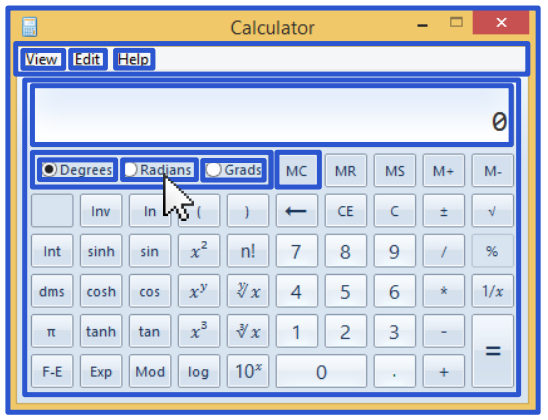
\includegraphics[scale=0.4]{GUI-ablak}
		\caption{A számológép alkalmazás grafikus felülete}
		\label{fig:GUI-ablak}
	\end{subfigure}
	~
	\begin{subfigure}[b]{0.5\textwidth}
		\centering
		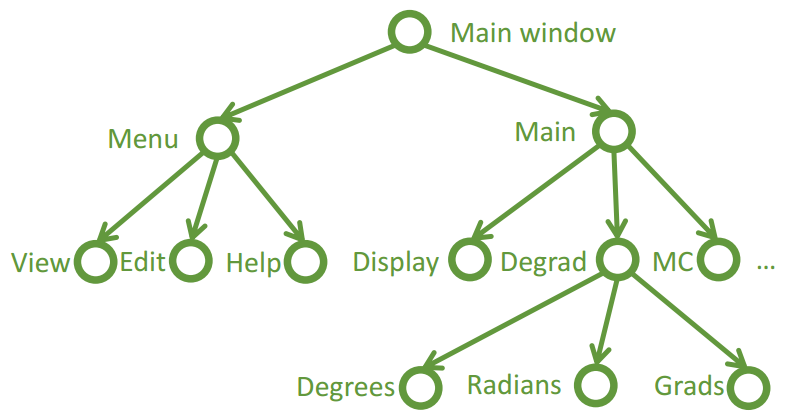
\includegraphics[scale=0.25]{GUI-hierarchia}
		\caption{A komponensek hierarchiája}
		\label{fig:GUI-hierarchia}
	\end{subfigure}
	\caption{A metróhálózatot ábrázoló gráf kiterjesztései}
\end{figure}

\begin{feladat}
	Mi történik, amikor egy alkalmazás ablakán kattintunk -- hogyan határozza meg a rendszer, hogy melyik komponensre kattintottunk?
\end{feladat}




%%%%%%%%%%%%%%%%%%%%%%%%%%%%%%%%%%%%%%%%%%%%%%%%%%%%%%%%%%%%%%%%%%%%%%%%%%%%%%%%%%%%%%%%%%%%%%%%%%%%




\section{Összefoglalás}

A fejezetben bemutattuk \fogalom{struktura-alapu-modellezes} motivációját, a használt formalizmusukat és azok alkalmazásait. Ismertettük \fogalomragozva{tipus}{típusok} fontosságát és a típusrendszer ábrázolásának lehetőségeit.

A következő fejezetekben a \fogalomragozva{viselkedes-alapu-modellezes}{viselkedés alapú modellezést} és annak formalizmusait mutatjuk be.

%%%%%%%%%%%%%%%%%%%%%%%%%%%%%%%%%%%%%%%%%%%%%%%%%%%%%%%%%%%%%%%%%%%%%%%%%%%%%%%%%%%%%%%%%%%%%%%%%%%%

\section{Kitekintés: technológiák és technikák\kieg}

Az alábbiakban bemutatunk néhány, a strukturális modellezés témaköréhez kapcsolódó gyakorlati technológiát, specifikációt és eszközt. Az itt felsorolt fogalmak nem részei a számonkérésnek, gyakran előkerülnek viszont a későbbi tanulmányok és munkák során, ezért mindenképpen érdemes legalább névről ismerni őket.

\subsection{Technológiák}

A gyakorlatban sokféle modellezési nyelvet és technológiát használnak. Ezek közül mutatunk be most azokat, amelyek a később tanulmányok során előkerülnek.

\subsubsection{UML}

Az \roviditesangolulkifejtve{UML} egy általános célú modellezési nyelv az~\cite{UML}. Az UML három fő diagramtípust definiál:

\begin{itemize}
	\item \emph{Structure Diagram:} strukturális modellek leírására. A \emph{Class Diagram} az osztályok (metamodell), míg az \emph{Object diagram} a példányok (modell) leírására alkalmas. A \emph{Composite Structure Diagram} egy rendszer struktúráját és a rendszer komponenseinek kapcsolatát mutatja be.
	\item \emph{Behaviour Diagram:} viselkedési modellek leírására, pl. a \emph{State Machine Diagram} segítségével állapotgépek az \emph{Activity Diagramon} folyamatok ábrázolhatók. A \emph{Behaviour Diagramek} között megkülönböztejük az \emph{Interaction Diagrameket}. Ezeknek szintén a viselkedés leírása a célja, de a hangsúly a vezérlés- és adatáramlás bemutatásán van. Ilyen pl. a \emph{Sequence Diagram} (szekvenciadiagram), amely az egyes objektumok közötti interakciót mutatja be üzenetek formájában.
\end{itemize}

\remofigscale{UML-diagram}{UML diagramok típusai és a közöttük lévő viszony osztálydiagramként ábrázolva~\cite{wiki:ISE}}{0.6}

Az UML nyelvvel részletesen foglalkozik a \szofttech tárgy. A nyelvről egy jó összefoglalót \az+\cite{uml-diagrams} oldal.

%\subsubsection{AADL}
%Az \roviditesangolulkifejtve{AADL} eredetileg repülőipari célokra fejlesztett architektúraleíró nyelv~\cite{AADL}.

\subsubsection{EMF}

Az Eclipse fejlesztőkörnyezet\footnote{\url{http://www.eclipse.org/}} saját modellezési keretrendszerrel rendelkezik, ez az \roviditesangolulkifejtve{EMF}. Az EMF metamodellező nyelve, az Ecore lehetővé teszi saját, ún. \roviditesteljesenkifejtve{DSL} definiálását. Az EMF mára több területen is \emph{de facto} modellezési keretrendszer.

Az Eclipse fejlesztőkörnyezettel és az EMF keretrendszerrel foglalkozik az \eat szabadon választható tárgy.

\subsection{Haladó strukturális modellezési technikák}

A struktúramodellek definiálására és fejlesztésére különböző technikák léteznek. Korábban tárgyaltuk a \fogalomangolul{top-down} és a \fogalomangolul{bottom-up} tervezést. Itt két további, általánosan alkalmazható technikát mutatunk be.

\subsubsection{Tervezési minták}

Az \fogalom{objektum-orientalt} tervezés során gyakran előforduló problémákra különböző \fogalomragozva{tervezesi-minta}{tervezési minták} (\fogalomragozva{tervezesi-minta}{design patterns}) léteznek. A tervezési minták között külön szerepet kapnak a rendszer struktúráját leíró \fogalomragozva{szerkezeti-minta}{szerkezeti minták} (\fogalomragozva{szerkezeti-minta}{structural patterns}). A tervezési mintákkal bővebben a \sznikak tárgy foglalkozik.

\subsubsection{Refaktoring}

A \fogalomragozva{dekompozicio}{dekompozícióhoz}, azaz \fogalomragozva{faktoring}{faktoringhoz} szorosan kapcsolódik a \fogalom{refaktoring} (\fogalomangolul{refaktoring}) fogalma~\cite{fowler2012refactoring}. Refaktoringon egy rendszert definiáló programkód vagy modell átalakítását értjük. A refaktoring lényege, hogy az átalakítás során a rendszer megfigyelhető működése változatlan marad, de a kapott programkód vagy modell érthetőbb, karbantarthatóbb lesz. Tipikus refaktoring műveletek pl. változók átnevezése, ismétlődő programrészletek megszüntetése (pl. külön metódusba vagy osztályba kiszervezéssel).

%\section{További technológiák}
%
%\subsubsection{SysML}
%
%A \roviditesangolulkifejtve{SysML} egy UML-alapú általános modellezési nyelv rendszertervezési célokra~\cite{SysML}. A SysML az UML egy részhalmazát bővíti ki és új diagramtípusokat is bevezet, pl. \emph{Requirement Diagram} követelmények és viszonyaik ábrázolására alkalmas.
%
%%\subsubsection{RDF}
%%
%%\roviditesangolulkifejtve{RDF}
%%
%%TODO erről is lesz szakirányos tárgy
%
%\subsubsection{AUTOSAR}
%
%Az \roviditesangolulkifejtve{AUTOSAR}~\cite{autosar} nagy autóipari gyártók és beszállítóik által fejlesztett szabványos architektúranyelv, amely az egyes hardver- és szoftverkomponensek együttműködése magas szinten definiálható. Az AUTOSAR konzorciumnak a \emph{Méréstechnika és Információs Rendszerek Tanszék} is tagja~\cite{autosar-attendees}.


\subsection{Struktúramodellező eszközök és vizualizáció}
\label{sec:eszkozok}

Gráfok automatikus megjelenítésére alkalmas pl. a GraphViz\footnote{\url{http://www.graphviz.org/}} programcsomag. Gráfok feldolgozására gyakran alkalmazzák az igraph\footnote{\url{http://igraph.org/}} programcsomagot. Manapság több gráfadatbázis-kezelő rendszer is elterjedt, pl. a Neo4j\footnote{\url{http://neo4j.com/}} és a Titan\footnote{\url{http://thinkaurelius.github.io/titan/}} rendszerek.

Gráfok manuális rajzolására szintén több eszköz elterjedt. Egyszerűen használható online felületet biztosít a draw.io\footnote{\url{http://draw.io/}} és az Arrow Tools\footnote{\url{http://www.apcjones.com/arrows/}}. A jegyzetben szereplő ábrák a yEd eszközzel\footnote{\url{https://www.yworks.com/products/yed}} készültek. Sok információt tartalmazó gráf esetén érdemes lehet vektorgrafikus rajzoló-, ill. prezentáló eszközök, pl. a Microsoft Visio vagy Microsoft PowerPoint alkalmazás.

%%%%%%%%%%%%%%%%%%%%%%%%%%%%%%%%%%%%%%%%%%%%%%%%%%%%%%%%%%%%%%%%%%%%%%%%%%%%%%%%%%%%%%%%%%%%%%%%%%%%

\section{Elméleti kitekintés\kieg}

A strukturális modellezésnek komoly matematikai eszköztára is van. Az alábbiakban ezekből mutatunk be néhány részletet.

%\subsection{Hipergráfok}
%
%A gráf adatmodell kiterjesztése a \fogalom{hipergraf}. A hipergráfban a \fogalomragozva{hiperel}{hiperélek} több csomópont között is futhatnak. Megkülönböztetünk irányított és irányítatlan hipergráfokat.
%
%Az irányítatlan hipergráfok egyszerűen leképezhetők \fogalomragozva{paros-graf}{páros gráffá}: a gráf egyik halmazában a hipergráf csomópontjainak, a másik halmazában a hiperéleknek veszünk fel egy pontot.
%

%\fogalom{kenyszer} + \rovidites{CSP}
%\todo[inline]{ábra}

%\subsection{Relációk}

%\subsection{Tudásreprezentáció}
%
%Predikátumkalkulus
%
%Elsőrendű logika

\subsection{Bináris relációk tulajdonságai}

%A \fogalom{tranzitiv-lezaras} fogalom jelentésének megértését segíti, ha \\
Egy $(D_1, D_2)$ halmazpáron értelmezett $R$ bináris relációt úgy definiálhatunk, mint ezen halmazok Descartes-szorzatának egy részhalmazát: $R \subseteq D_1 \times D_2$.

Hasznos ismerni a kétváltozós relációkon értelmezett tulajdonságokat~\cite{wiki:relacio}.

\begin{tipp}
	Az elnevezések egyezése nem véletlen, a \fogalom{ketvaltozos-relacio} egy alesete a \fogalom{relacio} fogalomnak.
\end{tipp}

%http://math.stackexchange.com/questions/65102/if-a-relation-is-symmetric-and-transitive-will-it-be-reflexive

\begin{definicio}
	Egy $S$ halmazon értelmezett $r$ kétváltozós reláció \fogalomragozva{reflexivitas}{reflexív}, ha bármely $a \in S$-re $r(a, a)$ teljesül.
\end{definicio}

\begin{definicio}
	Egy $S$ halmazon értelmezett $r$ kétváltozós reláció \fogalomragozva{szimmetria}{szimmetrikus}, ha bármely $a,b \in S$-re $r(a, b)$ teljesülése esetén $r(b, a)$ is teljesül. A nem szimmetrikus relációkat \fogalomragozva{aszimmetria}{aszimmetrikusnak} nevezzük.
\end{definicio}

\begin{definicio}
	Egy $S$ halmazon értelmezett $r$ kétváltozós reláció \fogalomragozva{tranzitivitas}{tranzitív}, ha bármely $a,b,c \in S$-re $r(a, b)$ és $r(b, c)$ teljesülése esetén $r(a, c)$ is teljesül.
\end{definicio}

\begin{pelda}
	\remofigscalefixed{tranzitivitas}{Az \emph{egyenlő} ($=$) és a \emph{kisebb} ($<$) relációk gráfon ábrázolva}{\yedscale}

	Tranzitív relációk:
	\begin{itemize}
	\item Az \emph{egyenlő} ($=$) és a \emph{kisebb} ($<$) relációk tranzitívak, mert
	\begin{itemize}
		\item $a = b$ és $b = c$ esetén $a = c$,
		\item $d < e$ és $e < f$ esetén $e < f$.
	\end{itemize}
	\Az+\ref{fig:tranzitivitas}. ábrán ábrázoltuk a fenti relációkat. Az $=$ reláció szimmetrikus, ezért irányítatlan gráffal, a $<$ reláció aszimmetrikus, ezért irányított gráffal reprezentálható.
	\end{itemize}

	Nem tranzitív relációk:
	\begin{itemize}
	\item A \emph{nemegyenlő} reláció ($\neq$) nem tranzitív, mert
	\begin{itemize}
		\item $a \neq b$ és $b \neq c$ esetén $a \neq c$ nem mindig áll fenn, például
		\item $1 \neq 2$ és $2 \neq 1$ esetén $1 \neq 1$ nem teljesül.
	\end{itemize}
	\item Személyek közötti $\mathit{őse}$ reláció tranzitív, mert $\mathit{őse}(a, b)$ és $\mathit{őse}(b, c)$ esetén $\mathit{őse}(a, c)$ is fennáll.
	\item Személyek közötti $\mathit{ismerőse}$ reláció nem tranzitív, mert $\mathit{ismerőse}(a, b)$ és $\mathit{ismerőse}(b, c)$ esetén nem garantált, hogy $\mathit{ismerőse}(a, c)$ fennáll.
	\end{itemize}
\end{pelda}

%%%%%%%%%%%%%%%%%%%%%%%%%%%%%%%%%%%%%%%%%%%%%%%%%%%%%%%%%%%%%%%%%%%%%%%%%%%%%%%%%%%%%%%%%%%%%%%%%%%%

\section{Ajánlott irodalom}

A gráfelmélettel behatóan foglalkozik a \bszketto tantárgy és Fleiner Tamás jegyzete~\cite{FleinerJegyzet}. Különböző gráfalgoritmusokat mutat be -- pl. \fogalom{legrovidebb-ut} és minimális összsúlyú \fogalom{feszitofa} keresésére -- az \algel tárgy. További keresőalgoritmusok a \mestersegesintelligencia tárgyban szerepelnek.

Olvasmányos összefoglalót nyújt az UML nyelvről Martin Fowler ,,UML distilled'' című könyve~\cite{fowler1997uml}.

A tulajdonsággráfokról egy jól érthető tudományos cikk Marko Rodriguez és Peter Neubauer munkája~\cite{Rodriguez2010}. Rodriguez a Titan elosztott gráfadatbázis-kezelő rendszer egyik fő fejlesztője, míg Neubauer a Neo4j gráfadatbázis-kezelőt fejlesztő cég alapítója (mindkét rendszert említettük \aref{sec:eszkozok}. szakaszban). Az elosztott gráfadatbázis alkalmazását, elméleti és gyakorlati kihívásait kiváló prezentációkban mutatja be~\cite{RodriguezSlides2012,RodriguezSlides2013}.

Barabási-Albert László magyar fizikus nemzetközileg elismert kutatója a komplex \fogalomragozva{halozat}{hálózatok} elméletének. Barabási ,,Behálózva'' című könyve közérthető stílusban mutatja be a hálózatok elemzésének elméleti kihívásait a kutatási eredmények gyakorlati jelentőségét~\cite{behalozva}. A szerzővel több interjú is készült.\footnote{\url{http://index.hu/tudomany/bal080429/}}\footnote{\url{http://index.hu/tudomany/2010/06/02/az_elso_cikk_utan_majdnem_leharaptak_a_fejunket/}}\footnote{\url{http://index.hu/tudomany/2015/02/20/az_nsa_primitiven_hasznalta_a_begyujtott_adatokat/}}

Az osztályok és prototípusok közötti elvi különbséget mutatja be Antero Taivalsaari, a Nokia Research fejlesztőjének cikke~\cite{DBLP:journals/joop/Taivalsaari97}.

%\roviditesangolulkifejtve{SQL}
%\fogalom{azonosito} (\fogalomragozva{elsodleges-kulcs}{elsődleges kulcsok})
